% Options for packages loaded elsewhere
\PassOptionsToPackage{unicode}{hyperref}
\PassOptionsToPackage{hyphens}{url}
\PassOptionsToPackage{dvipsnames,svgnames,x11names}{xcolor}
%
\documentclass[
]{article}
\usepackage{amsmath,amssymb}
\usepackage{lmodern}
\usepackage{iftex}
\ifPDFTeX
  \usepackage[T1]{fontenc}
  \usepackage[utf8]{inputenc}
  \usepackage{textcomp} % provide euro and other symbols
\else % if luatex or xetex
  \usepackage{unicode-math}
  \defaultfontfeatures{Scale=MatchLowercase}
  \defaultfontfeatures[\rmfamily]{Ligatures=TeX,Scale=1}
\fi
% Use upquote if available, for straight quotes in verbatim environments
\IfFileExists{upquote.sty}{\usepackage{upquote}}{}
\IfFileExists{microtype.sty}{% use microtype if available
  \usepackage[]{microtype}
  \UseMicrotypeSet[protrusion]{basicmath} % disable protrusion for tt fonts
}{}
\makeatletter
\@ifundefined{KOMAClassName}{% if non-KOMA class
  \IfFileExists{parskip.sty}{%
    \usepackage{parskip}
  }{% else
    \setlength{\parindent}{0pt}
    \setlength{\parskip}{6pt plus 2pt minus 1pt}}
}{% if KOMA class
  \KOMAoptions{parskip=half}}
\makeatother
\usepackage{xcolor}
\usepackage[margin=1in]{geometry}
\usepackage{graphicx}
\makeatletter
\def\maxwidth{\ifdim\Gin@nat@width>\linewidth\linewidth\else\Gin@nat@width\fi}
\def\maxheight{\ifdim\Gin@nat@height>\textheight\textheight\else\Gin@nat@height\fi}
\makeatother
% Scale images if necessary, so that they will not overflow the page
% margins by default, and it is still possible to overwrite the defaults
% using explicit options in \includegraphics[width, height, ...]{}
\setkeys{Gin}{width=\maxwidth,height=\maxheight,keepaspectratio}
% Set default figure placement to htbp
\makeatletter
\def\fps@figure{htbp}
\makeatother
\setlength{\emergencystretch}{3em} % prevent overfull lines
\providecommand{\tightlist}{%
  \setlength{\itemsep}{0pt}\setlength{\parskip}{0pt}}
\setcounter{secnumdepth}{-\maxdimen} % remove section numbering
\usepackage{graphics}
\usepackage{xparse}
\usepackage{tcolorbox}
\usepackage{wrapfig}
\usepackage{helvet}
\usepackage{sectsty}
\usepackage{fancyhdr}
\usepackage{xpatch}
\usepackage{booktabs}
\pagestyle{fancy}
\definecolor{gssmidblue}{RGB}{32, 115, 188}
\definecolor{dfeheadingblue}{RGB}{16, 79, 117}
\renewcommand{\familydefault}{\sfdefault}
\allsectionsfont{\color{dfeheadingblue}}
\sectionfont{\color{dfeheadingblue}\fontsize{24}{30}\selectfont}
\fancyhead[C]{*** Note that this is a draft document and does not contain genuine data ***}
\fancyhead[L,R]{}
\fancyfoot[R]{\nouppercase{\emph{\rightmark}}}
\fancyfoot[L]{\nouppercase{\emph{\leftmark}}}
\fancyfoot[C] {}
\renewcommand{\headrulewidth}{0pt}
\renewcommand{\footrulewidth}{2pt}
\futurelet\TMPfootrule\def\footrule{{\color{gssmidblue}\TMPfootrule}}
\usepackage{booktabs}
\usepackage{longtable}
\usepackage{array}
\usepackage{multirow}
\usepackage{wrapfig}
\usepackage{float}
\usepackage{colortbl}
\usepackage{pdflscape}
\usepackage{tabu}
\usepackage{threeparttable}
\usepackage{threeparttablex}
\usepackage[normalem]{ulem}
\usepackage{makecell}
\usepackage{xcolor}
\ifLuaTeX
  \usepackage{selnolig}  % disable illegal ligatures
\fi
\IfFileExists{bookmark.sty}{\usepackage{bookmark}}{\usepackage{hyperref}}
\IfFileExists{xurl.sty}{\usepackage{xurl}}{} % add URL line breaks if available
\urlstyle{same} % disable monospaced font for URLs
\hypersetup{
  colorlinks=true,
  linkcolor={Maroon},
  filecolor={Maroon},
  citecolor={Blue},
  urlcolor={blue},
  pdfcreator={LaTeX via pandoc}}

\author{}
\date{\vspace{-2.5em}}

\begin{document}


\includegraphics[width=0.25\linewidth]{"images/Department_for_Education.png"}
\vspace{2.4cm}

\hypertarget{la-secondary-school-places-scorecard-for-wokingham}{%
\section{LA Secondary School Places Scorecard for
Wokingham}\label{la-secondary-school-places-scorecard-for-wokingham}}

\vspace{3.2cm}
\vspace*{\fill}
\color{dfeheadingblue}{\hrule}
\color{black}

\hypertarget{introduction}{%
\subsection{Introduction}\label{introduction}}

This document presents school places figures for Wokingham covering
quantity of places available, forecast accuracy of pupil projections,
places allocated by preference, new places allocated by school quality
and cost per place. It is intended to provide a downloadable, printable
document of figures for individual Local Authorities as an alternative
to our online dashboard (available
\href{https://department-for-education.shinyapps.io/la-school-places-scorecards/}{here}).

\vspace{12pt}

\newpage

\hypertarget{quantity}{%
\subsection{Quantity}\label{quantity}}

\makebox[1.00\linewidth]{
\centering


\begin{tcolorbox}[colback=gssmidblue, 
 leftright skip=0.1cm,
 coltext=white, 
 halign=left, 
 fontupper={\Huge \bfseries},
 fontlower={\large \bfseries},
 sharp corners, 
 colframe=gssmidblue,
 width=0.49\linewidth,
 boxrule=0pt,
 equal height group=introbox
 ]
£59million
\tcblower
Total primary and secondary basic need funding 2011 to 2022
\end{tcolorbox}


\begin{tcolorbox}[colback=gssmidblue, 
 leftright skip=0.1cm,
 coltext=white, 
 halign=left, 
 fontupper={\Huge \bfseries},
 fontlower={\large \bfseries},
 sharp corners, 
 colframe=gssmidblue,
 width=0.49\linewidth,
 boxrule=0pt,
 equal height group=introbox
 ]
21\%
\tcblower
Growth in secondary pupil numbers 2009/10 to 2021/22
\end{tcolorbox}
}

\hypertarget{places-created-since-200910-places-planned-to-202122-and-estimated-place-pressure-in-202122}{%
\subsubsection{Places created since 2009/10, places planned to 2021/22
and estimated place pressure in
2021/22}\label{places-created-since-200910-places-planned-to-202122-and-estimated-place-pressure-in-202122}}

A local authority can have both `spare places' and `additional places
needed' due to localised or specific year group demand

\makebox[1.0\linewidth]{
\centering
\begin{tcolorbox}[colback=gssmidblue, 
 leftright skip=0.1cm,
 coltext=white, 
 halign=left, 
 fontupper={\Huge \bfseries},
 fontlower={\large \bfseries},
 sharp corners, 
 colframe=gssmidblue,
 width=0.49\linewidth,
 boxrule=0pt,
 equal height group=quanbox
 ]
70
\tcblower
Estimated additional secondary places to meet demand in 2021/22 
\end{tcolorbox}
\begin{tcolorbox}[colback=gssmidblue, 
 leftright skip=0.1cm,
 coltext=white, 
 halign=left, 
 fontupper={\Huge \bfseries},
 fontlower={\large \bfseries},
 sharp corners, 
 colframe=gssmidblue,
 width=0.49\linewidth,
 boxrule=0pt,
 equal height group=quanbox
 ]
5\%
\tcblower
Estimated percentage of spare secondary places in 2021/22
\end{tcolorbox}
}

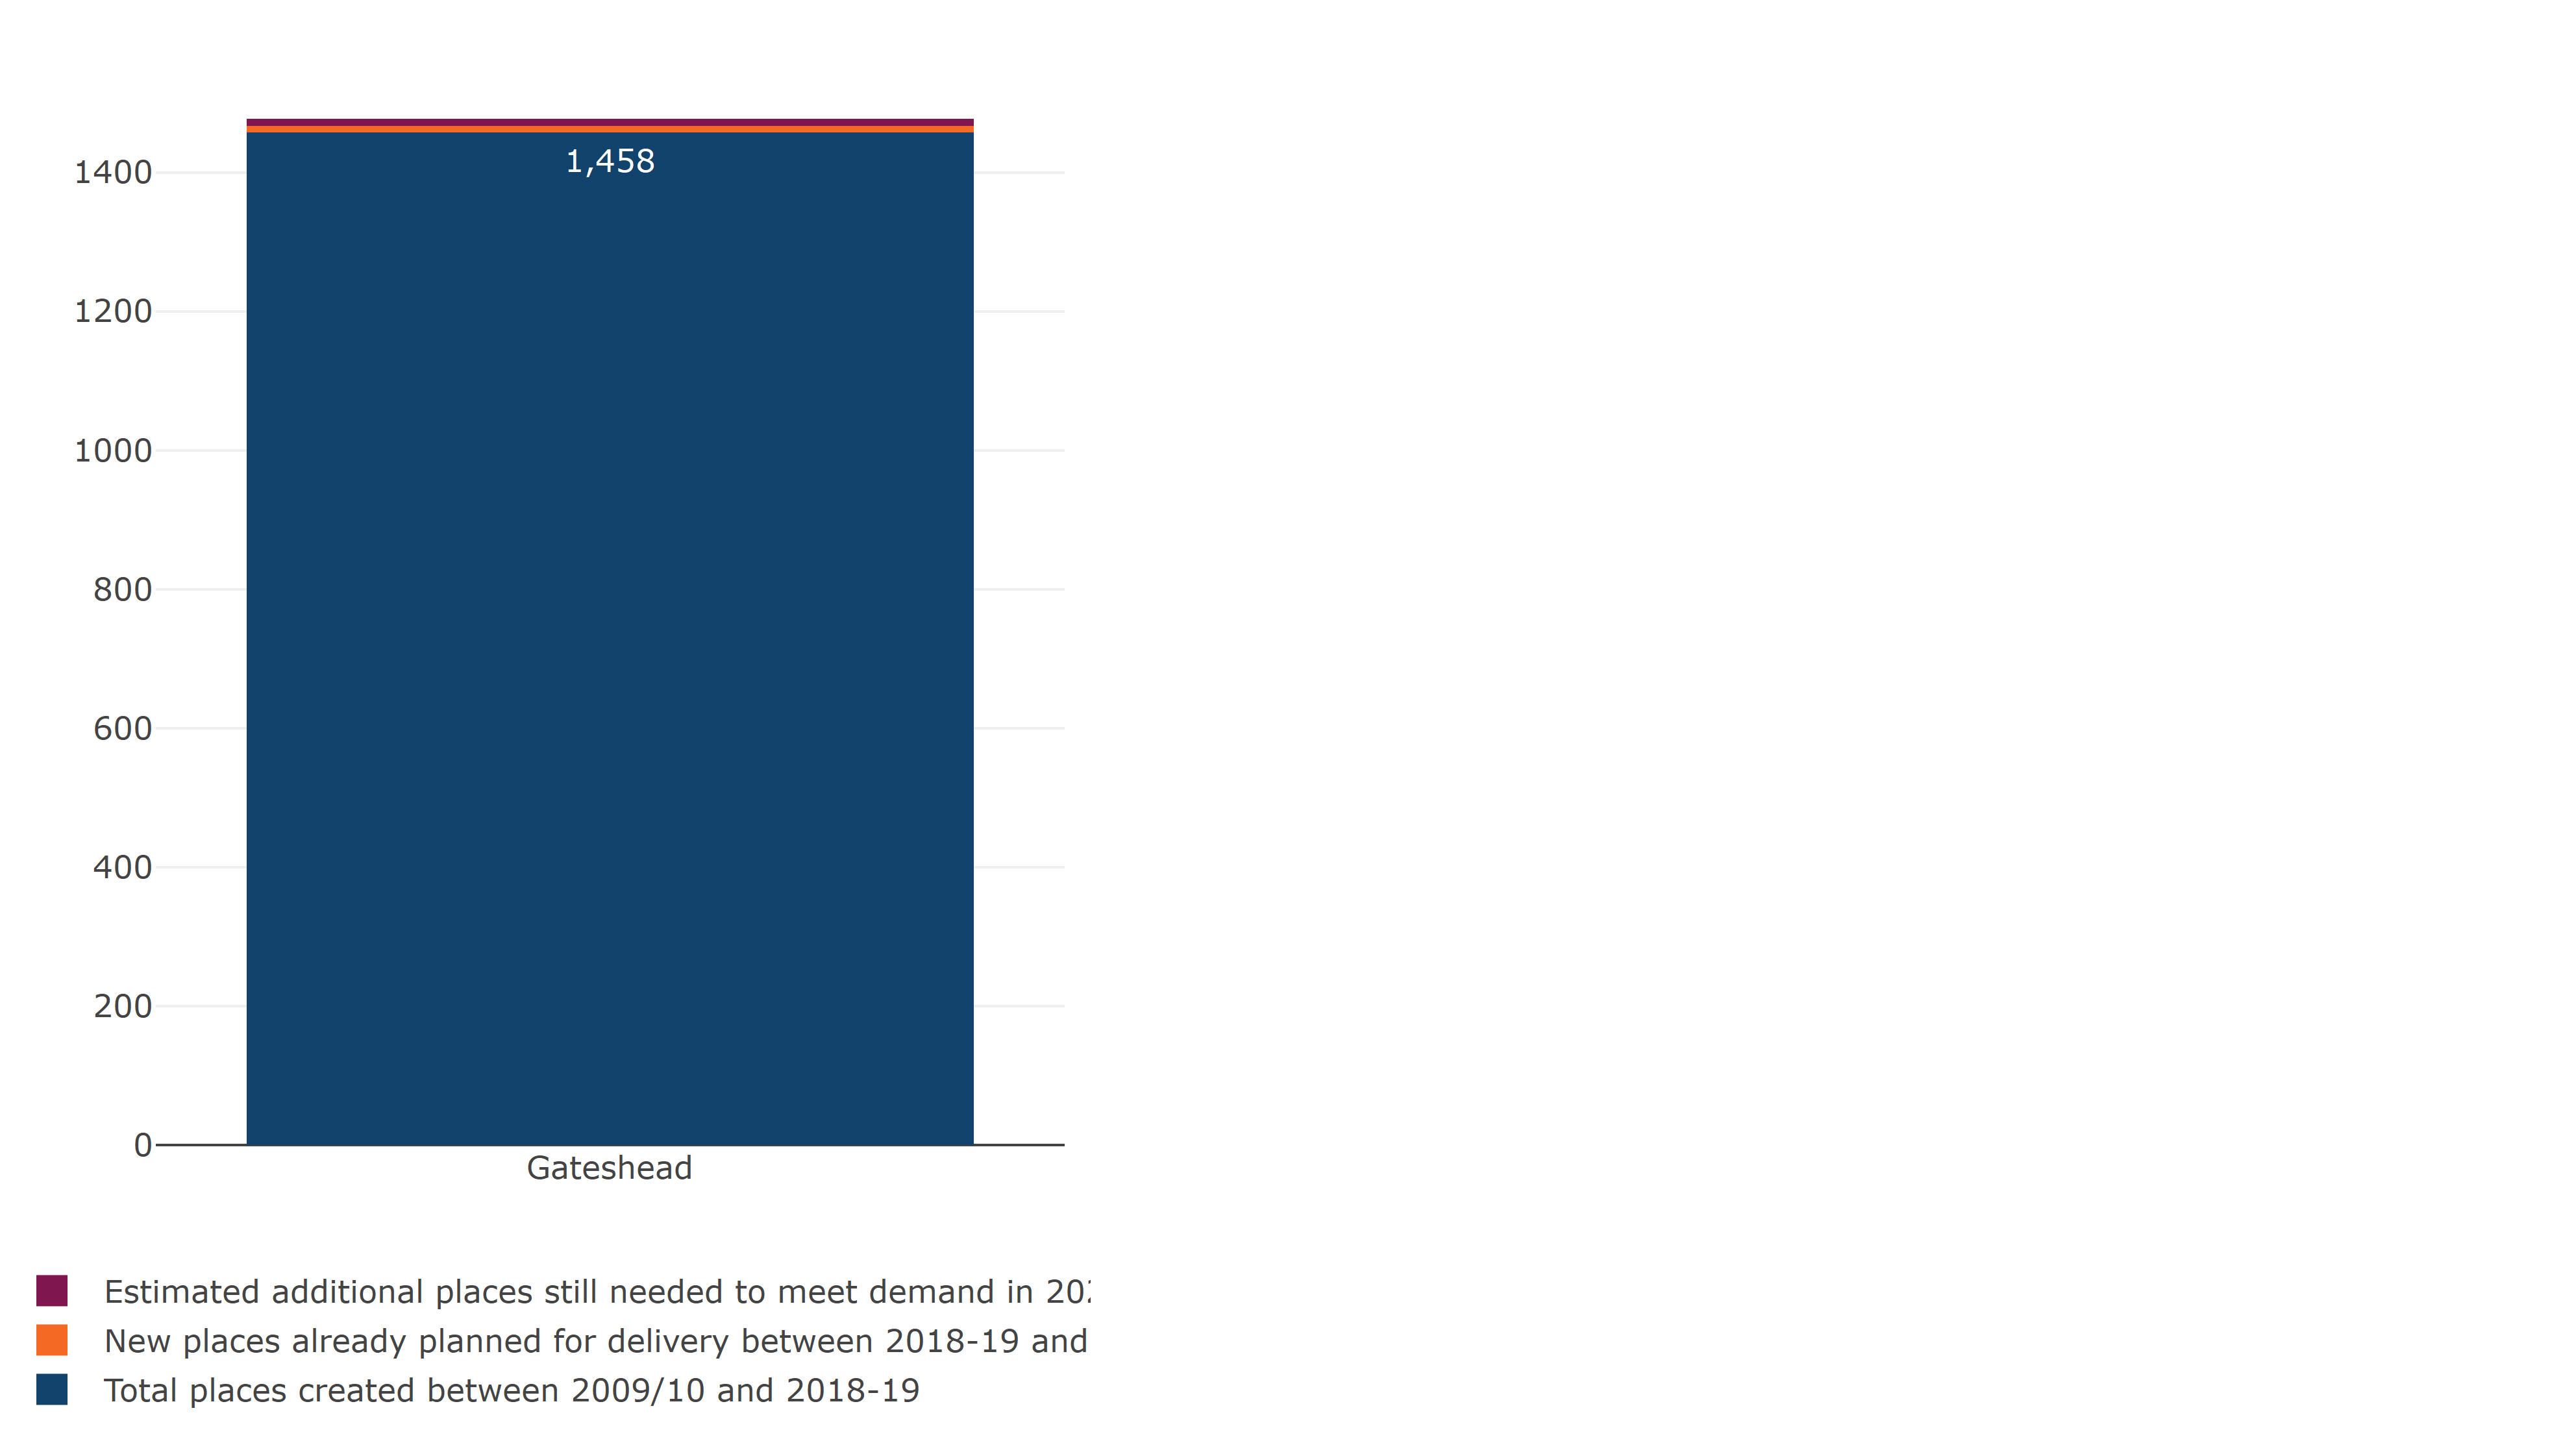
\includegraphics[width=1\linewidth]{Summary_scorecard_files/figure-latex/quantity_b-1}

\newpage

\hypertarget{forecast-accuracy}{%
\subsection{Forecast Accuracy}\label{forecast-accuracy}}

\hypertarget{forecast-accuracy-of-pupil-projections-for-202122-made-one-year-and-three-years-previously}{%
\subsubsection{Forecast accuracy of pupil projections for 2021/22, made
one year and three years
previously}\label{forecast-accuracy-of-pupil-projections-for-202122-made-one-year-and-three-years-previously}}

The shaded area in each chart ending at the thick vertical line shows
the forecasting accuracy for Wokingham. The starting point is 0, an
accurate score, indicated by a dotted line. A shared area to the right
of 0 indicates an overestimate, a shared area to the left of 0 indicates
an underestimate.\\
The grey dashed lines show the 25th and 75th percentile score for all
local authorities.

\begin{tabular}{p{0.48\linewidth} p{0.48\linewidth} }\bf\large\color{dfeheadingblue} One year ahead: -0.2\% \ & \bf\large\color{dfeheadingblue} Three years ahead: -4.9\% \ \\Underestimate of pupil numbers, larger underestimation than at least 75\% of local authorities&Underestimate of pupil numbers, larger underestimation than at least 75\% of local authorities \\\end{tabular}

\includegraphics[width=0.5\linewidth]{Summary_scorecard_files/figure-latex/forecast22-1}
\includegraphics[width=0.5\linewidth]{Summary_scorecard_files/figure-latex/forecast22-2}

\begin{tabular}{p{0.48\linewidth} p{0.48\linewidth} }\footnotesize \centering 
\begin{tabular}{lllll}
\toprule
Min & 25th centile & Median & 75th centile & Max\\
\midrule
-1.8\% & +0.5\% & +1.3\% & +1.9\% & +5.4\%\\
\bottomrule
\end{tabular}
&\footnotesize \centering 
\begin{tabular}{lllll}
\toprule
Min & 25th centile & Median & 75th centile & Max\\
\midrule
-7.7\% & +1.4\% & +2.9\% & +4.4\% & +15.8\%\\
\bottomrule
\end{tabular}
\end{tabular}

\newpage

\hypertarget{preference}{%
\subsection{Preference}\label{preference}}

\hypertarget{proportion-of-applicants-who-received-an-offer-of-one-of-their-top-three-preference-schools-for-september-2019-entry}{%
\subsubsection{Proportion of applicants who received an offer of one of
their top three preference schools for September 2019
entry}\label{proportion-of-applicants-who-received-an-offer-of-one-of-their-top-three-preference-schools-for-september-2019-entry}}

\makebox[1.0\linewidth]{
\centering
\begin{tcolorbox}[colback=gssmidblue, 
 leftright skip=0.1cm,
 coltext=white, 
 halign=left, 
 fontupper={\Huge \bfseries},
 fontlower={\large \bfseries},
 sharp corners, 
 colframe=gssmidblue,
 width=0.49\linewidth,
 boxrule=0pt ,
 equal height group=prefbox
 ]
93\%
\tcblower
Percentage of applicants who received an offer of one of their top three preferred secondary schools in England
\end{tcolorbox}

\begin{tcolorbox}[colback=gssmidblue, 
 leftright skip=0.1cm,
 coltext=white, 
 halign=left, 
 fontupper={\Huge \bfseries},
 fontlower={\large \bfseries},
 sharp corners, 
 colframe=gssmidblue,
 width=0.49\linewidth,
 boxrule=0pt,
 equal height group=prefbox
 ]
93.8\%
\tcblower
Percentage of applicants who received an offer of one of their top three preferred secondary schools in Wokingham
\end{tcolorbox}
}

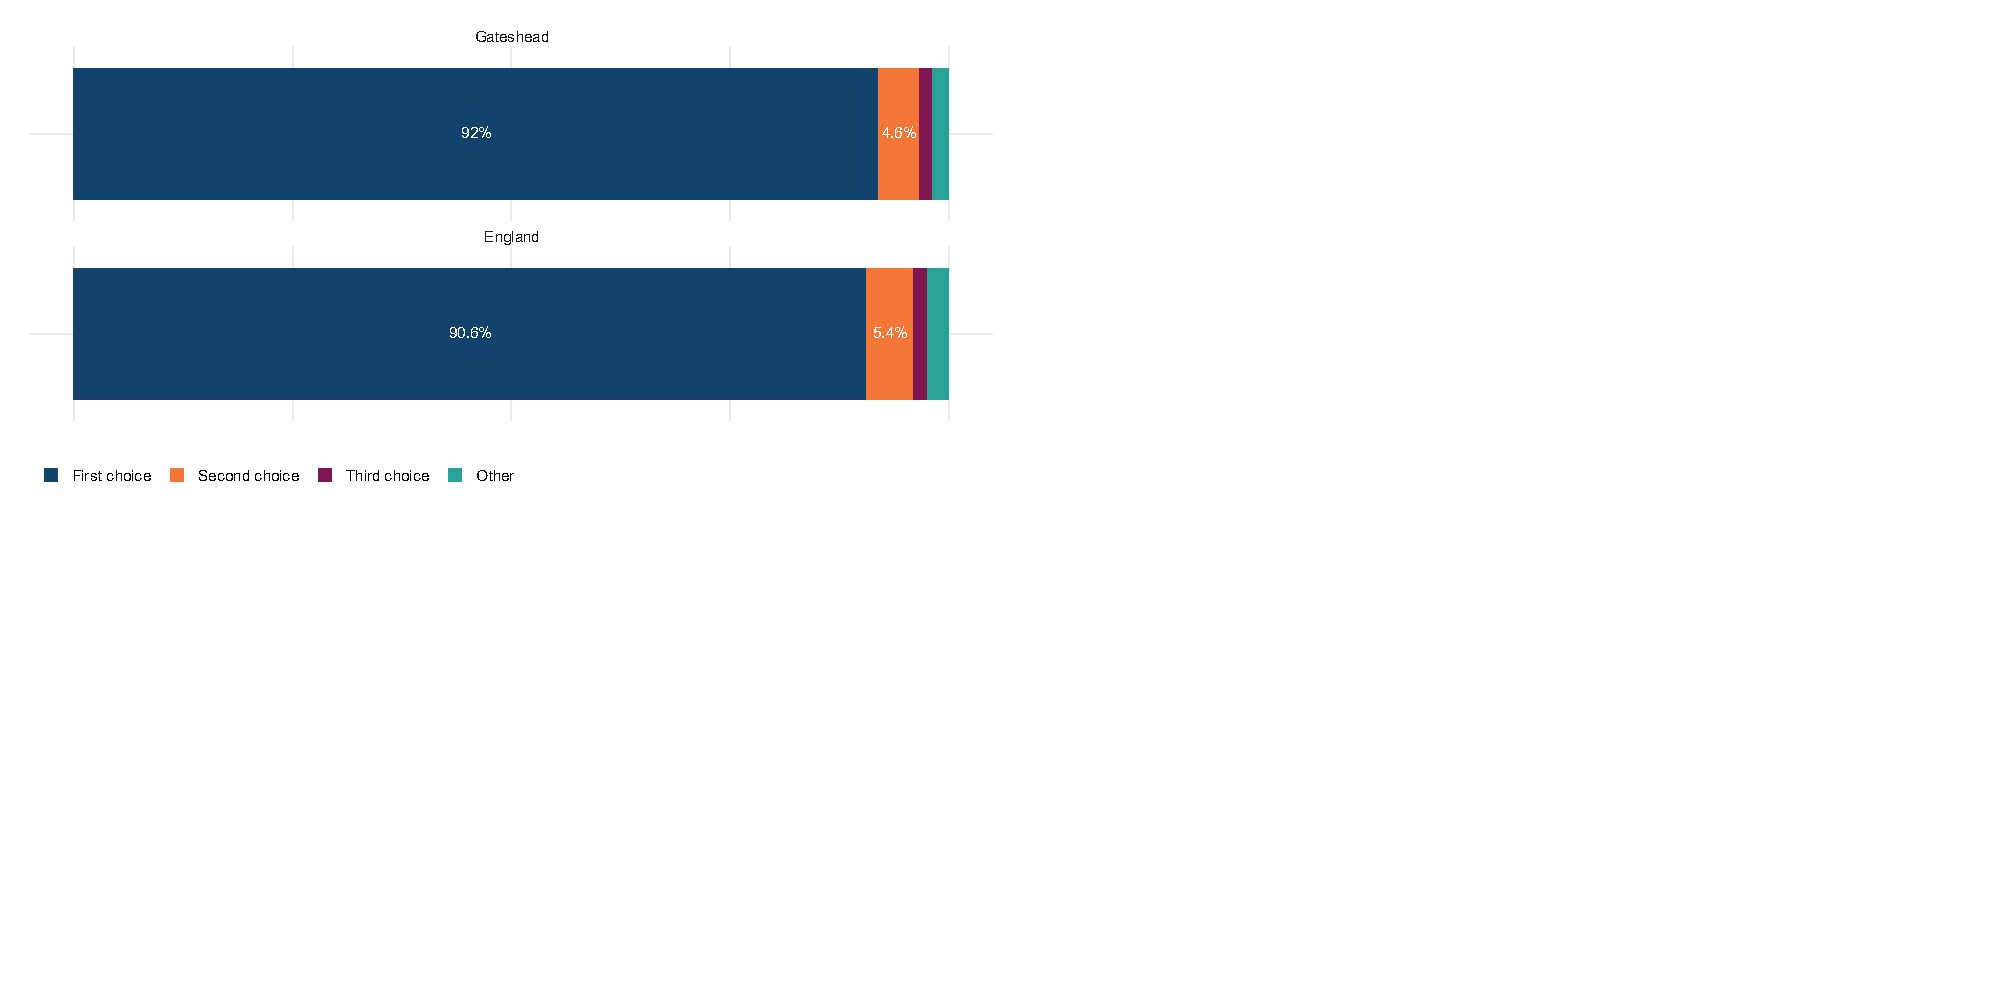
\includegraphics[width=1\linewidth]{Summary_scorecard_files/figure-latex/preference_barchart-1}

\newpage

\hypertarget{quality}{%
\subsection{Quality}\label{quality}}

\hypertarget{quality-of-places-created-between-201718-and-201819-based-on-ofsted}{%
\subsubsection{Quality of places created between 2017/18 and 2018/19,
based on
Ofsted:}\label{quality-of-places-created-between-201718-and-201819-based-on-ofsted}}

\makebox[1.0\linewidth]{
\centering
\begin{tcolorbox}[colback=gssmidblue, 
 leftright skip=0.1cm,
 coltext=white, 
 halign=left, 
 fontupper={\Huge \bfseries},
 fontlower={\large \bfseries},
 sharp corners, 
 colframe=gssmidblue,
 width=0.32\linewidth,
 boxrule=0pt,
 equal height group=qualbox
 ]
88.2\%
\tcblower
Percentage of new places created in good and outstanding  secondary schools in England
\end{tcolorbox}
\begin{tcolorbox}[colback=gssmidblue, 
 leftright skip=0.1cm,
 coltext=white, 
 halign=left, 
 fontupper={\Huge \bfseries},
 fontlower={\large \bfseries},
 sharp corners, 
 colframe=gssmidblue,
 width=0.32\linewidth,
 boxrule=0pt,
 equal height group=qualbox 
 ]
100\%
\tcblower
Percentage of new places created in good and outstanding secondary schools in Wokingham
\end{tcolorbox}
\begin{tcolorbox}[colback=gssmidblue, 
 leftright skip=0.1cm,
 coltext=white, 
 halign=left, 
 fontupper={\Huge \bfseries},
 fontlower={\large \bfseries},
 sharp corners, 
 colframe=gssmidblue,
 width=0.32\linewidth,
 boxrule=0pt,
 equal height group=qualbox
 ]
1
\tcblower
LA Rank out of 114 LAs that created new places between 2017/18 and 2018/19 (ranks can be tied)
\end{tcolorbox}
}

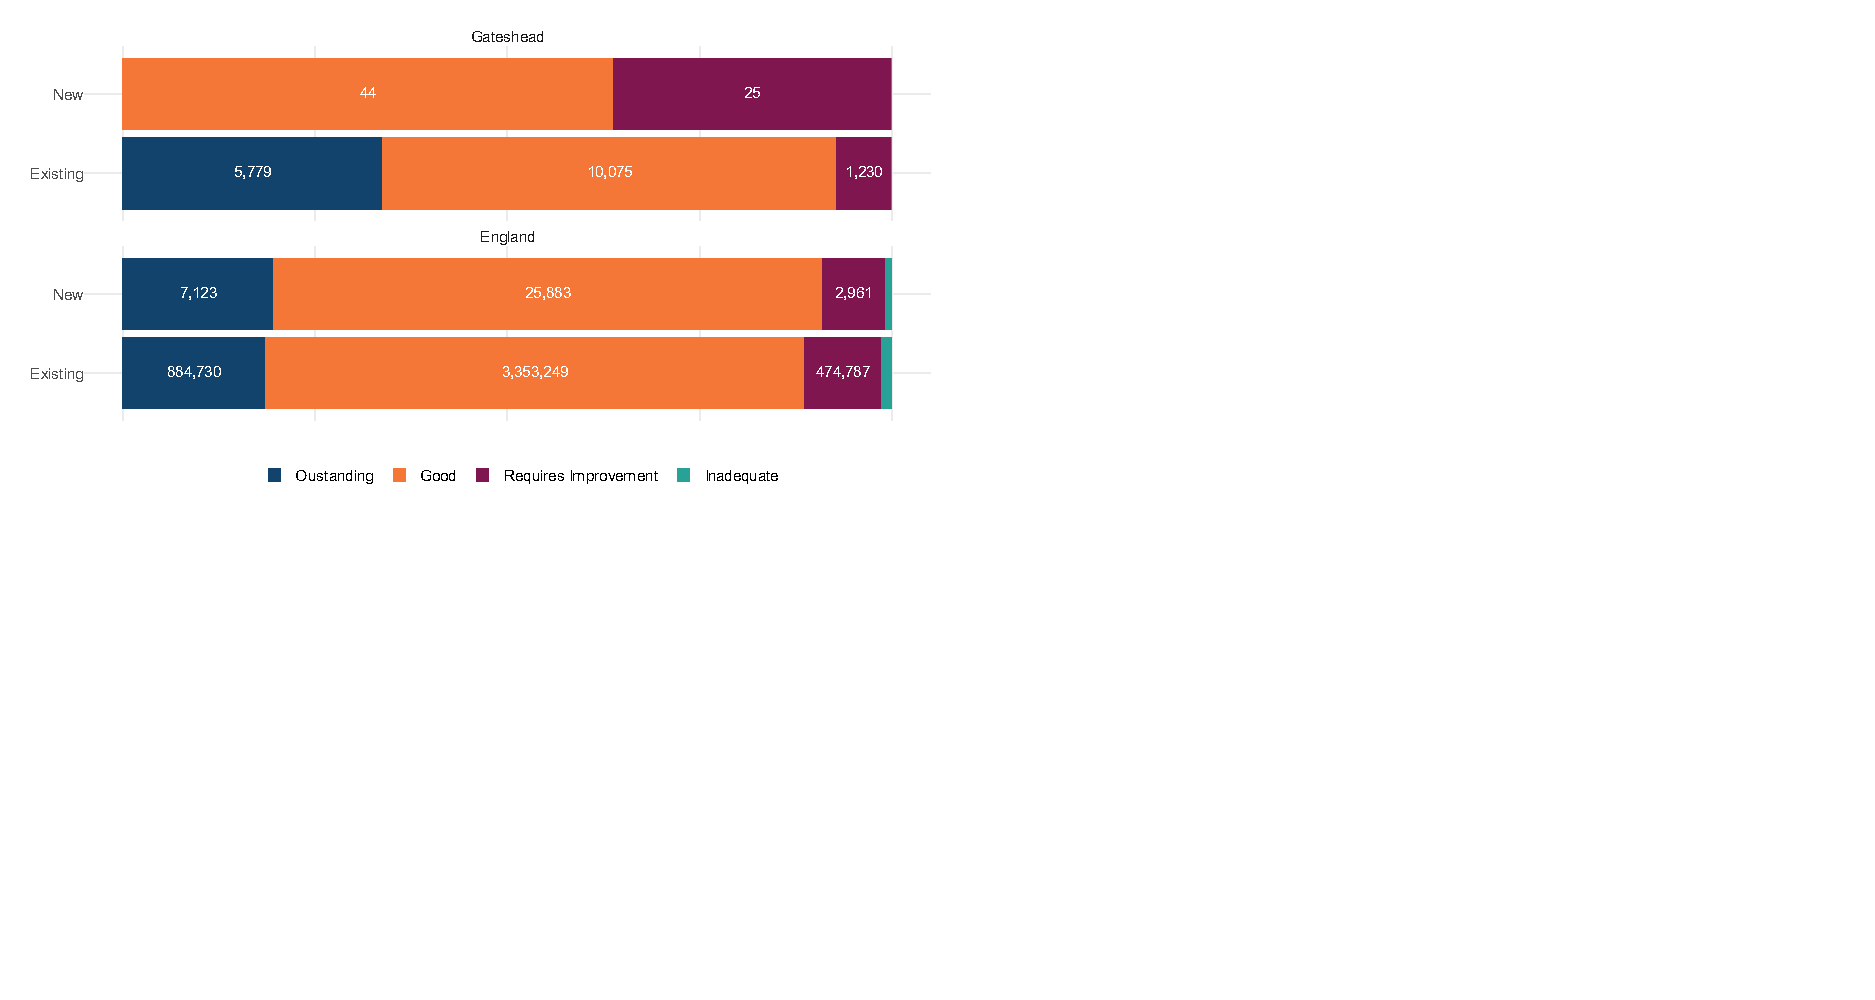
\includegraphics[width=0.92\linewidth]{Summary_scorecard_files/figure-latex/quality_chart-1}

New places with no rating = NA

\newpage

\hypertarget{cost}{%
\subsection{Cost}\label{cost}}

\hypertarget{average-cost-of-additional-mainstream-school-places}{%
\subsubsection{Average cost of additional mainstream school
places}\label{average-cost-of-additional-mainstream-school-places}}

Based on local authority reported projects between 2015/16 and 2017/18
adjusted for inflation and regional variation

\makebox[1.0\linewidth]{
\centering
\begin{tcolorbox}[colback=gssmidblue, 
 leftright skip=0.1cm,
 coltext=white, 
 halign=left, 
 fontupper={\Huge \bfseries},
 fontlower={\large \bfseries},
 sharp corners, 
 colframe=gssmidblue,
 width=0.32\linewidth,
 boxrule=0pt,
 equal height group=costbox
 ]
0
\tcblower
Permanent secondary expansion projects in England
\end{tcolorbox}

\begin{tcolorbox}[colback=gssmidblue, 
 leftright skip=0.1cm,
 coltext=white, 
 halign=left, 
 fontupper={\Huge \bfseries},
 fontlower={\large \bfseries},
 sharp corners, 
 colframe=gssmidblue,
 width=0.32\linewidth,
 boxrule=0pt,
 equal height group=costbox
 ]
0
\tcblower
Temporary secondary expansion projects in England
\end{tcolorbox}

\begin{tcolorbox}[colback=gssmidblue, 
 leftright skip=0.1cm,
 coltext=white, 
 halign=left, 
 fontupper={\Huge \bfseries},
 fontlower={\large \bfseries},
 sharp corners, 
 colframe=gssmidblue,
 width=0.32\linewidth,
 boxrule=0pt,
 equal height group=costbox
 ]
1
\tcblower
New secondary schools projects in England
\end{tcolorbox}
}

\hypertarget{average-cost-per-place-for-permanent-temporary-and-new-school-projects}{%
\subsubsection{Average cost per place for permanent, temporary and new
school
projects}\label{average-cost-per-place-for-permanent-temporary-and-new-school-projects}}

Region column shows England averages, adjusted for regional location
factors

\begin{tabular}{lll}
\toprule
Type & England & North East\\
\midrule
Permanent Expansion & £23,775 & -\\
Temporary Expansion & £9,248 & -\\
New school & £24,929 & £31,954\\
\bottomrule
\end{tabular}

\newpage
\vspace*{\fill}
\color{dfeheadingblue}{\hrule}
\color{black}

\hypertarget{contact}{%
\subsection{Contact}\label{contact}}

\begin{quote}
Pupil place planning team

Publication:
\href{https://explore-education-statistics.service.gov.uk/find-statistics/local-authority-school-places-scorecards}{Explore
Education Statistics: Local authority school places scorecards}

Dashboard:
\href{https://department-for-education.shinyapps.io/la-school-places-scorecards}{LA
School Places Scorecards}

Email:
\href{mailto:SCAP.PPP@education.gov.uk}{\nolinkurl{SCAP.PPP@education.gov.uk}}

This document was produced using the
\href{https://github.com/dfe-analytical-services}{DfE Analytical
Services} Rmarkdown template, which is available on GitHub as part of
our
\href{https://github.com/dfe-analytical-services/shiny-template}{R-Shiny
data dashboard template}.
\end{quote}

\href{https://www.gov.uk/government/organisations/department-for-education}{
\includegraphics[width=0.50\linewidth]{"images/Department_for_Education_long.png"}}

\end{document}
